\begin{figure*}[t]
  \centering
  
  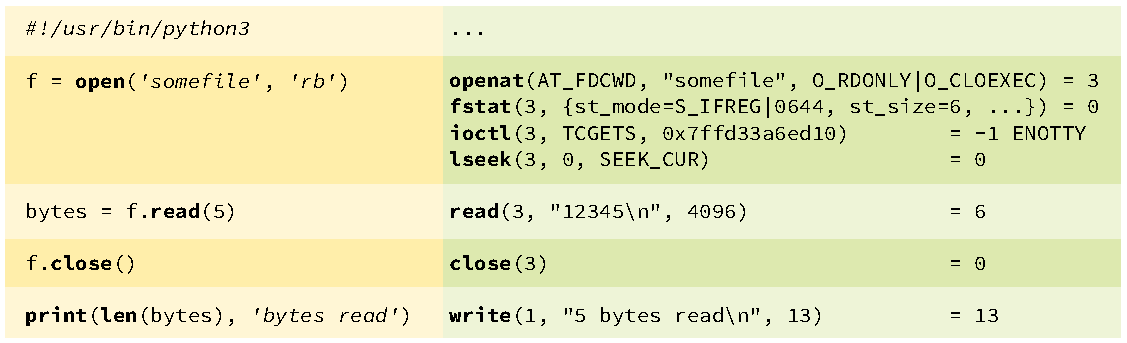
\includegraphics[scale=.8]{../images/sample-listing}
  \caption{Beispielhaftes Python-Programm (link) und dessen \strace-Ausgabe (rechts) \newline
  \emph{Anmerkung:} Die \strace-Ausgabe wurde um den relevanten Anteil gekürzt
  }
  \label{fig:sample-listing}
\end{figure*}

\section{\strace{} in Aktion}

\subsection{Analyse eines einfachen Programms}

Genug der Theorie. In diesem Abschnitt wollen wir uns die Ausgabe von \strace{} anhand eines
einfachen Beispiels ansehen. \autoref{fig:sample-listing} zeigt links ein kurzes Python-Skript.
Python wurde deshalb gewählt, weil es auch ohne Spezialkenntnisse leicht vertändlich ist --
deutlich einfacher als die Programmiersprache C.

Ein Shellskript ist zur Darstellung von \strace ungeeignet, da es in der Regel sehr viele externe
Programme aufruft, sog. \emph{Kindprozesse}. Gerade zu Beginn eines neu gestarteten Programmes 
werden jedoch viele Systemaufrufe durchgeführt (Laden von Bibliotheken, Übersetzungsdateien),
die für Laien erstmal schwer verständlich sind. 


Auf der rechten Seite von \autoref{fig:sample-listing} wird die unveränderte Ausgabe von \strace{}
dargestellt. Allerdings wurde nur der wesentliche Teil gelistet.

Um das Beispiel nachvollziehen zu können, starten wir das Programm folgenermaßen in einer Shell:

\begin{verbatim}
  % strace notfound.py > output.txt
\end{verbatim}

Die Ausgabeumleitung in \texttt{output.txt} wird vorgenommen damit sich die Ausgabe vom Programm
und von \strace{} nicht vermischen. Zunächst werden einige hundert Zeilen Output erzeugt die für
uns irrelevant sind. Bevor der Python-Interpreter das Programm ausführt muss erstmal der
Python-Interpreter initialisiert werden, müssen Bibliothken vom Betriebssystem geladen werden und
muss das eigentliche Skript gelesen werden. Bei einem kompilierten C-Programm\footnote{oder
natürlich auch einem Pascal- oder Go-Programm, also jeder Programmiersprache, die in ein
Maschinenprogramm übersetzt wird} wäre dieser Anteil deutlich kürzer aber dennoch relativ groß.

Die Kunst besteht darin, den eigentlichen Start des Teils des Programms zu finden, der uns
interessiert. Am besten liest man von unten nach oben. Oder man leitet die Ausgabe von \strace{}
ein eine Datei um -- wie das geht erfahren wir im nächsten Kapitel -- und sucht im Texteditor nach
einem bekannten String: Das kann eine (bekannte) Ausgabe sein oder den Namen der Datei, die
geöffnet wird.

Das Beispiel wurde so formatiert, dass die Zeilen des Programms und die korrespondierenden 
Systemaufrufe klar erkennbar sind. Dennoch nachfolgend ein paar Erklärungen.

\begin{itemize}
  \item Zunächst wird die Datei \texttt{somefile} zum Lesen geöffnet. Daraus resultiert
    ein Systemaufruf \texttt{open()}. Der Python-Interpreter verwendet das etwas modernere
    \texttt{openat()}, welches zusätzlich noch ermöglicht, anzugeben, wie relative Pfade
    behandelt werden.

    Das Ergebnis ist der \emph{Dateideskriptor} mit der Nummer 3, der bei den folgenden
    Systemaufrufen dann immer als erstes Argument angegeben wird. Dieser Dateideskriptor ist wichtig
    um die Aufrufe den verschiedenen Dateien zuordnen zu können!

    Anschließend werden Metainformationen zur Datei gelelesen, dafür wird \texttt{fstat()}
    verwendet. Zur Metainformation gehören die Größe und Zugriffsrechte der Datei. Der Aufruf
    \texttt{ioctl()} prüft, ob die Datei ein Terminal ist, \texttt{lseek()} setzt die Position
    des Lesezeigers auf den Anfang\footnote{Im Prinzip sind diese Operationen für das Programm
    gar nicht erforderlich. Das ist ein Problem der Abstraktion in der Informatik: Je "`einfacher"'
    die Programmiersprache gehalten ist, je mehr automatisch passiert, deso schwieriger wird es,
    das Verhalten des Systems auf unterster Ebene zu verstehen und deso mehr Dinge werden
    erledigt, die gar nicht erledigt werden müssten.}.

  \item Nun werden mit \texttt{f.read()} maximal 5 Bytes gelesen. Der Python-Interpreter hingegen
    puffert intern, versucht also einen ganzen Puffer von 4096 Bytes zu lesen und bekommt tatsächlich 6 Bytes. Dies ist der Rückgabewert des Systemaufrufs \texttt{read()}.

  \item \texttt{close()} gibt den Dateideskriptor 3 wieder frei.

  \item \texttt{write()} schreibt die Meldung "`5 Bytes read"' auf die Standardausgabe. Gemäß
    \autoref{tab:errno} ist der Dateideskriptor 1 die Standardausgabe.
\end{itemize}

\minisec{Fehlerfall}

Nun löschen wir die Datei \texttt{somefile,} so dass sie nicht vorhanden ist\footnote{Deshalb heißt
das Programm ja auch \texttt{notfound.py}.} und starten das Programm erneut. Die wesentliche
Zeile der \strace-Ausgabe sieht wie folgt aus:

\begin{lstlisting}
openat(AT_FDCWD, "somefile", O_RDONLY|O_CLOEXEC) = -1 ENOENT (Datei oder Verzeichnis nicht gefunden)
\end{lstlisting}

Hier ist klar erkennbar, dass die Datei nicht geöffnet wurde, weil die nicht exisistiert. Statt
einem (positiven) Dateideskriptor gibt \texttt{openat()} den Fehlercode $-1$ zurück, der gemäß
\href{http://man7.org/linux/man-pages/man3/errno.3.html}{\emph{errno(3)}} bzw. \autoref{tab:errno} 
„Datei oder Verzeichnis nicht gefunden“ bedeutet. Dieser Fehlertext ist praktischerweise in der
Ausgabe von \strace{} auch gleich mit enthalten.

Danach kommen jede Menge Fehlerausgaben, die einfach deshalb in \strace{} auftauchen, weil sich das
Python-Programm mit einer Ausnahme beendet.


